\documentclass[tikz,border=6pt]{standalone}
\usepackage{newtxtext,newtxmath}
\usetikzlibrary{arrows.meta,positioning,fit,calc}
\definecolor{paperink}{HTML}{3F4852}
\definecolor{papergray}{HTML}{EEF1F4}
\definecolor{paperamber}{HTML}{A66A14}
\definecolor{papergreen}{HTML}{287A4D}
\begin{document}
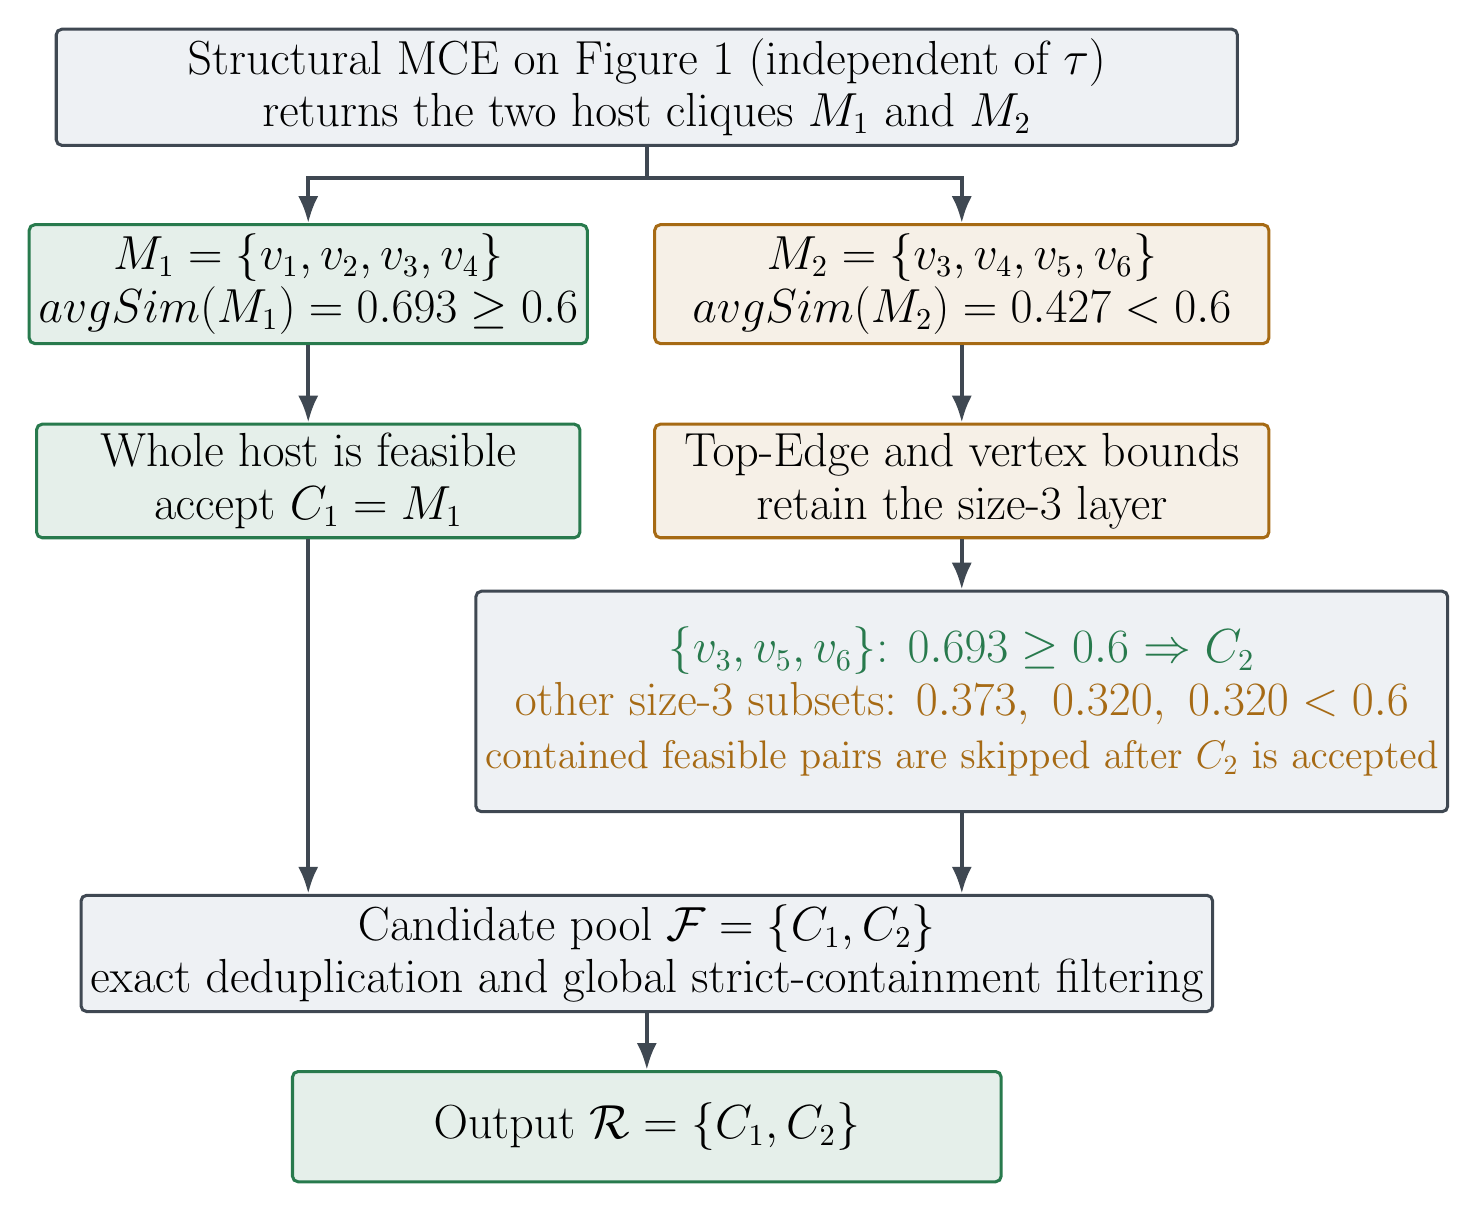
\begin{tikzpicture}[
  font=\fontsize{16}{19}\selectfont,
  >=Latex,
  box/.style={draw=paperink, rounded corners=2pt, line width=1.1pt,
    align=center, minimum height=14mm, fill=white},
  structural/.style={fill=papergray},
  bounded/.style={fill=paperamber!10, draw=paperamber},
  accepted/.style={fill=papergreen!12, draw=papergreen},
  arrow/.style={->, line width=1.5pt, draw=paperink}
]
\node[box, structural, minimum width=150mm] (bk) at (8,0)
  {Structural MCE on Figure 1 (independent of $\tau$)\\
   returns the two host cliques $M_1$ and $M_2$};

\node[box, accepted, minimum width=69mm] (m1) at (3.7,-2.5)
  {$M_1=\{v_1,v_2,v_3,v_4\}$\\$\operatorname{avgSim}(M_1)=0.693\geq0.6$};
\node[box, bounded, minimum width=78mm] (m2) at (12,-2.5)
  {$M_2=\{v_3,v_4,v_5,v_6\}$\\$\operatorname{avgSim}(M_2)=0.427<0.6$};
\draw[arrow] (bk.south) -- ++(0,-4mm) -| (m1.north);
\draw[arrow] (bk.south) -- ++(0,-4mm) -| (m2.north);

\node[box, accepted, minimum width=69mm]
  (c1) at (3.7,-5.0) {Whole host is feasible\\accept $C_1=M_1$};
\node[box, bounded, minimum width=78mm]
  (bounds) at (12,-5.0) {Top-Edge and vertex bounds\\retain the size-$3$ layer};
\draw[arrow] (m1) -- (c1);
\draw[arrow] (m2) -- (bounds);

\node[box, structural, minimum width=78mm, minimum height=28mm]
  (layer) at (12,-7.8)
  {{\color{papergreen}$\{v_3,v_5,v_6\}$: $0.693\geq0.6$ $\Rightarrow C_2$}\\
   {\color{paperamber}other size-$3$ subsets: $0.373,\ 0.320,\ 0.320<0.6$}\\
   {\fontsize{14}{17}\selectfont\color{paperamber}contained feasible pairs are skipped after $C_2$ is accepted}};
\draw[arrow] (bounds) -- (layer);

\node[box, structural, minimum width=118mm] (filter) at (8,-11.0)
  {Candidate pool $\mathcal F=\{C_1,C_2\}$\\
   exact deduplication and global strict-containment filtering};
\draw[arrow] (c1.south) -- (c1.south |- filter.north);
\draw[arrow] (layer.south) -- (layer.south |- filter.north);
\node[box, accepted, minimum width=90mm]
  (out) at (8,-13.2) {Output $\mathcal R=\{C_1,C_2\}$};
\draw[arrow] (filter) -- (out);
\end{tikzpicture}
\end{document}
